\documentclass[conference]{IEEEtran}
\IEEEoverridecommandlockouts
% The preceding line is only needed to identify funding in the first footnote. If that is unneeded, please comment it out.
%Template version as of 6/27/2024

\usepackage{cite}
\usepackage{amsmath,amssymb,amsfonts}
\usepackage{algorithmic}
\usepackage{graphicx}
\usepackage{textcomp}
\usepackage{xcolor}
\def\BibTeX{{\rm B\kern-.05em{\sc i\kern-.025em b}\kern-.08em
    T\kern-.1667em\lower.7ex\hbox{E}\kern-.125emX}}


%后加的包
%\usepackage{booktabs}
\usepackage{multirow}
\usepackage[T1]{fontenc}


\begin{document}

\title{3D ISAR Reconstruction of Asteroids via Temporal Geometric Features and Visibility-Aware Modeling\\

\thanks{This work was supported by the National Natural Science Foundation of
	China under Grant 62227901.}
}

\author{\IEEEauthorblockN{1\textsuperscript{st} Zhicheng Xie}
\IEEEauthorblockA{\textit{School of Information and Electronics} \\
\textit{Beijing Institute of Technology}\\
Beijing, China \\
zhichengxieleo@163.com}
\and
\IEEEauthorblockN{2\textsuperscript{nd} Peiyao Liu}
\IEEEauthorblockA{\textit{School of Information and Electronics} \\
\textit{Beijing Institute of Technology}\\
Beijing, China \\
peiyao2429@163.com}
\and
\IEEEauthorblockN{3\textsuperscript{rd} Zhen Wang}
\IEEEauthorblockA{\textit{School of Information and Electronics} \\
\textit{Beijing Institute of Technology}\\
Beijing, China \\
wangzhenbit@163.com}
}

\maketitle

\begin{abstract}
This document is a model and instructions for \LaTeX.
This and the IEEEtran.cls file define the components of your paper [title, text, heads, etc.]. *CRITICAL: Do Not Use Symbols, Special Characters, Footnotes, 
or Math in Paper Title or Abstract.
\end{abstract}

\begin{IEEEkeywords}
ISAR, asteroid, rotation parameter estimation, 3D reconstruction.
\end{IEEEkeywords}

\section{Introduction}
This document is a model and instructions for \LaTeX.

\section{Ground-Based Radar Observation Geometry and Signal Model}

In this section, 

\subsection{Observation Geometry}\label{Observation}

Due to the combined effects of self-gravity, rotation, and long-term collisional evolution, the global shape of most asteroids can be approximated as a triaxial ellipsoid, which is adopted in this paper as the initial geometric baseline for 3D reconstruction.

First, an asteroid intrinsic coordinate system, denoted as $O-xyz$, is established with its origin at the target's center of mass. The $x$-axis aligns with the ellipsoid's major axis (with a semi-axis length of $a$), while the $y$- and $z$-axes are orthogonally determined by the right-hand rule (with semi-axis lengths of $b$ and $c$, respectively). Within this intrinsic coordinate system, the 3D geometric morphology of the initial reference ellipsoid is uniquely characterized by the shape covariance matrix $\mathbf{\Sigma}_0 = \text{diag}(a^2, b^2, c^2)$.

Most asteroids can be regarded as freely rotating rigid bodies without external torques. Assuming simple rotation about the principal axis of inertia (which aligns with the $z$-axis of the intrinsic coordinate system), the spin period $T$ and the pole direction remain constant during the observation. Let the scalar angular velocity be $\omega = 2\pi/T$, yielding the angular velocity vector $\boldsymbol{\omega} = [0, 0, \omega]^T$. The pole direction is uniquely determined by the ecliptic longitude $\lambda$ and ecliptic latitude $\beta$. To establish the observation geometry, the ecliptic coordinate system is mapped to the asteroid intrinsic coordinate system, as illustrated in Fig. \ref{fig_coordinate}.

\begin{figure}[htbp]
	\centerline{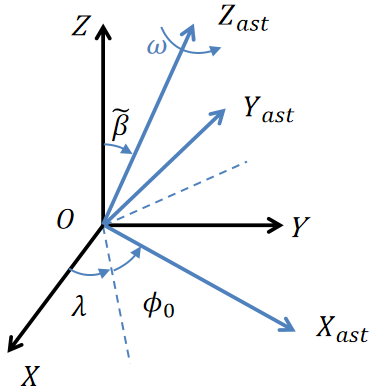
\includegraphics[width=0.4\columnwidth]{fig_coordinate.png}}
	\caption{Ecliptic to asteroid intrinsic coordinate transformation.}
	\label{fig_coordinate}
\end{figure}

Let $\mathbf{P}_{ecl}(t)$ denote the radar position vector in the ecliptic frame, obtained from the Jet Propulsion Laboratory (JPL) Horizons system. Through successive Euler angle rotations based on $\lambda$, $\beta$, and the initial observation phase $\phi_0$, its coordinates in the asteroid intrinsic coordinate system, denoted as $\mathbf{P}_{ast}(t)$, can be calculated via \cite{Gao2026}:
\begin{equation}
	\mathbf{P}_{ast}(t) = \mathbf{R}_z(\omega t + \phi_0) \mathbf{R}_y(\widetilde{\beta}) \mathbf{R}_z(\lambda) \cdot \mathbf{P}_{ecl}(t)
\end{equation}
where $\widetilde{\beta} = 90^\circ - \beta$ represents the ecliptic co-latitude, and $\mathbf{R}_z(\cdot)$ and $\mathbf{R}_y(\cdot)$ denote the fundamental rotation matrices around the $z$-axis and $y$-axis, respectively.

Finally, let $\mathbf{u}_{r}(t)$ be the unit line-of-sight (LOS) vector pointing from the asteroid's center of mass toward the radar in the intrinsic coordinate system, which is defined as $\mathbf{u}_{r}(t) = \mathbf{P}_{ast}(t) / \|\mathbf{P}_{ast}(t)\|= \big[ u_x(t), u_y(t), u_z(t) \big]^T$. 

Notably, under the far-field assumption for ground-based radar observations of asteroids, the incident wave can be approximated as a plane wave, implying that the unit LOS vector $\mathbf{u}_{r}(t)$ remains spatially identical across the entire target body. This time-varying unit vector characterizes the dynamic observation perspective and serves as the fundamental projection axis for the subsequent radar echo modeling and 3D reconstruction.

\subsection{Echo Signal Model and Image Formation}\label{Echo}

For an asteroid rotating as a rigid body, the ground-based radar echo is modeled as the coherent summation of reflections from all visible surface scattering points. Assuming the macroscopic translational bulk motion $R_0(t)$ of the asteroid's center of mass has been fully compensated via standard envelope alignment and dechirp processing of the Wideband Linear Frequency Modulated (LFM) signals, the final focused ISAR image $I(f_d, r)$ in the range-Doppler domain can be analytically formulated as the superposition of 2D Point Spread Function (PSF) responses:
\begin{equation}
	I(f_d, r) = \sum_{i \in \mathbb{V}} \sigma_i \cdot h \left( f_d - f_{di}, r - r_i \right)
\end{equation}
where $\mathbb{V}$ denotes the set of all visible scattering points considering self-occlusion, and $\sigma_i$ is the backscattering coefficient of the $i$-th point, which is modeled using a Lambertian scattering law (i.e., $\sigma_i \propto \cos^2\theta_i$, with $\theta_i$ being the local incidence angle). The function $h(\cdot, \cdot)$ represents the 2D radar PSF, whose mainlobe dimensions are determined by the theoretical Doppler resolution $\rho_d = 1 / T_{obs}$ and range resolution $\rho_r = c / (2B)$, with $c$ being the speed of light, $T_{obs}$ the coherent integration time, and $B$ the signal bandwidth.

Geometrically, the ideal 2D projection coordinates $(f_{di}, r_i)$ of the $i$-th scatterer at 3D position $\mathbf{r}_i$ are mapped via:
\begin{equation}
	\begin{cases}
		f_{di}(t) = \frac{2}{\lambda_{wav}} \langle \mathbf{u}_r(t) \times \boldsymbol{\omega}, \mathbf{r}_i \rangle \\
		r_i(t) = \langle \mathbf{u}_r(t), \mathbf{r}_i \rangle
	\end{cases}
	\label{fdi_ri}
\end{equation}
where $\lambda_{wav}$ is the radar wavelength.

Rewriting this point-to-pixel mapping in a compact matrix form, we define the $2 \times 3$ linear projection matrix $\mathbf{H}(t)$:
\begin{equation}
	\mathbf{H}(t) = 
	\begin{bmatrix}
		\frac{2}{\lambda_{wav}} \left( \mathbf{u}_r(t) \times \boldsymbol{\omega} \right)^T \\
		\mathbf{u}_r^T(t)
	\end{bmatrix}
\end{equation}

Consequently, for a triaxial asteroid characterized by the initial 3D shape covariance matrix $\mathbf{\Sigma}_0$, its global theoretical envelope in the 2D ISAR image is strictly the affine transformation of $\mathbf{\Sigma}_0$ under $\mathbf{H}(t)$. The projected 2D covariance matrix $\mathbf{\Sigma}_{RD}(t)$ characterizing the global ISAR contour is directly derived as:
\begin{equation}
	\mathbf{\Sigma}_{RD}(t) = \mathbf{H}(t)\,\mathbf{\Sigma}_0\,\mathbf{H}^T(t) =
	\begin{bmatrix}
		c_{11}(t) & c_{12}(t) \\
		c_{12}(t) & c_{22}(t)
	\end{bmatrix}
\end{equation}
where
\begin{equation}
	\begin{cases}
		c_{11}(t) = \left( \frac{4\pi}{\lambda_{wav} T} \right)^2 \left( a^2 u_y^2(t) + b^2 u_x^2(t) \right) \\
		c_{12}(t) = c_{21}(t) = \frac{4\pi}{\lambda_{wav} T} u_x(t) u_y(t) \left( a^2 - b^2 \right) \\
		c_{22}(t) = a^2 u_x^2(t) + b^2 u_y^2(t) + c^2 u_z^2(t)
	\end{cases}
\end{equation}

By directly extracting the elements of $\mathbf{\Sigma}_{RD}(t)$, the tangible macroscopic geometric features of the envelope on the Range-Doppler plane can be analytically formulated. Specifically, the theoretical Doppler width $\hat{L}_{d}(t)$, the range length $\hat{L}_{r}(t)$, and the tilt angle $\hat{\theta}(t)$ of the ISAR envelope relative to the Doppler frequency domain are strictly determined by the matrix elements as follows:
\begin{equation}
	\begin{cases}
		\hat{L}_{d}(t) = 2\sqrt{c_{11}(t)} \\
		\hat{L}_{r}(t) = 2\sqrt{c_{22}(t)} \\
		\hat{\theta}(t) = \frac{1}{2} \arctan \left( \frac{2 c_{12}(t)}{c_{11}(t) - c_{22}(t)} \right)
	\end{cases}
\end{equation}

\section{Proposed Method}

In this section, 


\subsection{Rotation Parameter Estimation}\label{Rotation}

To address the challenge of inaccurate scale priors for non-cooperative targets, this section proposes a scale-invariant estimation strategy based on the consistency of dynamic envelope evolution. By matching the temporal evolution trends of geometric features, this approach effectively decouples the rotation parameters $\Omega = \{T, \phi_0, \lambda, \beta\}$ from the absolute dimensions of the target.

In practical ISAR observations, the theoretical macroscopic features defined previously cannot be directly obtained due to the inevitable LOS self-occlusion effect. Therefore, the actual geometric features must be extracted from partially occluded 2D images.

Specifically, assume that a sequence of $N$ ISAR images is obtained at discrete observation times $\{t_k\}_{k=1}^N$. The target region is extracted via morphological processing, from which the second-order central moments are computed to derive the observed envelope tilt angle sequence $\boldsymbol{\theta} = \{\theta(t_k)\}_{k=1}^N$. Concurrently, by projecting valid pixels onto the Doppler and range axes, the Doppler width sequence $\mathbf{L}_d = \{L_d(t_k)\}_{k=1}^N$ and range length sequence $\mathbf{L}_r = \{L_r(t_k)\}_{k=1}^N$ are obtained.

The rotation parameters are estimated via a scale-invariant cost function $J(\Omega)$. For the tilt angle sequence, the cosine distance is employed to measure the temporal discrepancy, where a factor of 2 resolves the $180^\circ$ ambiguity inherent in geometric symmetry. For the Doppler width and range length sequences, the Pearson Correlation Coefficient (PCC) is utilized to quantify the similarity of their temporal evolution trends. This formulation explicitly decouples the rotation parameters from the absolute geometric scale based on temporal dynamics.

The final cost function is formulated as:
\begin{equation}
	\begin{split}
		J(\Omega) &= w_1 \left( 1 - \frac{1}{N} \sum_{k=1}^N \cos \Big( 2 \big( \theta(t_k) - \hat{\theta}(t_k; \Omega) \big) \Big) \right) \\
		&\quad + w_2 \big( 1 - \text{Corr}(\mathbf{L}_d, \hat{\mathbf{L}}_d(\Omega)) \big) \\
		&\quad + w_3 \big( 1 - \text{Corr}(\mathbf{L}_r, \hat{\mathbf{L}}_r(\Omega)) \big)
	\end{split}
\end{equation}
where $\hat{\theta}(t_k; \Omega)$, $\hat{\mathbf{L}}_d(\Omega)$, and $\hat{\mathbf{L}}_r(\Omega)$ denote the theoretical sequences predicted by the parameter set $\Omega$; $\text{Corr}(\cdot, \cdot)$ denotes the Pearson correlation operator, and $w_1, w_2, w_3$ are weighting coefficients. Considering that the self-occlusion effect along the LOS attenuates the reliability of range length observations, $w_3$ is typically assigned a smaller value compared to $w_1$ and $w_2$.

Due to the highly non-linear and multi-modal nature of $J(\Omega)$, gradient-based methods are prone to local optima. Consequently, a Genetic Algorithm (GA) is employed to explore the non-convex search space and identify the global optimum.

\subsection{Shape Parameter Inversion}\label{Shape}

Shape Inversion


\section{Simulation Experiments}

In this section, computer simulation experiments are conducted to validate the aforementioned analysis and demonstrate the effectiveness of the proposed method.

\subsection{Simulation Setup}

A realistic 3D mesh model of asteroid 1999~JV6, obtained from the \textit{3D Asteroid Catalogue}, is utilized as the ground truth in our simulations. The model is scaled to dimensions of 44.39~m, 21.92~m, and 20.88~m along the X, Y, and Z axes, respectively. The corresponding coordinate ranges are defined as $x \in [-22.37, 22.02]$~m, $y \in [-11.71, 10.21]$~m, and $z \in [-10.85, 10.03]$~m.

The ground-based radar operates in the X-band with a center frequency of 9.6~GHz. To accommodate the asteroid's scale, the system bandwidth is set to 150~MHz, yielding a range resolution of 1~m. The coherent integration time for each ISAR frame is 100~s, corresponding to a Doppler resolution of 0.01~Hz.

The asteroid rotation parameters are configured as follows: the spin period is 9.0~h (32,400~s). The rotation axis orientation is specified in the ecliptic coordinate system with longitude $\lambda=23.3^{\circ}$ and latitude $\beta=45.0^{\circ}$. The initial rotation phase is set to $\phi_0=60.0^{\circ}$.

To account for realistic radar receiver characteristics, a noise model is incorporated into the simulated ISAR intensity images. A constant additive thermal noise floor is globally injected across all observation epochs to simulate a realistic ground-based radar system. The noise power is calibrated such that the peak signal-to-noise ratio (SNR) across the entire observation sequence is 16~dB.

To simulate a realistic observation trajectory, the time-varying geometry is derived from the 2027 flyby ephemeris of asteroid 1999~AN10. A total of 18 ISAR frames are generated over two distinct observation epochs: $t \in [0, 8]$~h and $t \in [59.2, 67.2]$~h. Each epoch provides 9 uniformly sampled frames at 1-hour intervals. This dual-epoch scheme ensures sufficient geometric diversity to mitigate self-occlusion effects. To intuitively illustrate this, the corresponding radar LOS directions in the asteroid intrinsic coordinate system are plotted in Fig.~\ref{fig_radar_los}. The simulation parameters are summarized in Table~\ref{tab_sim_params}.

\begin{figure}[htbp]
	\centerline{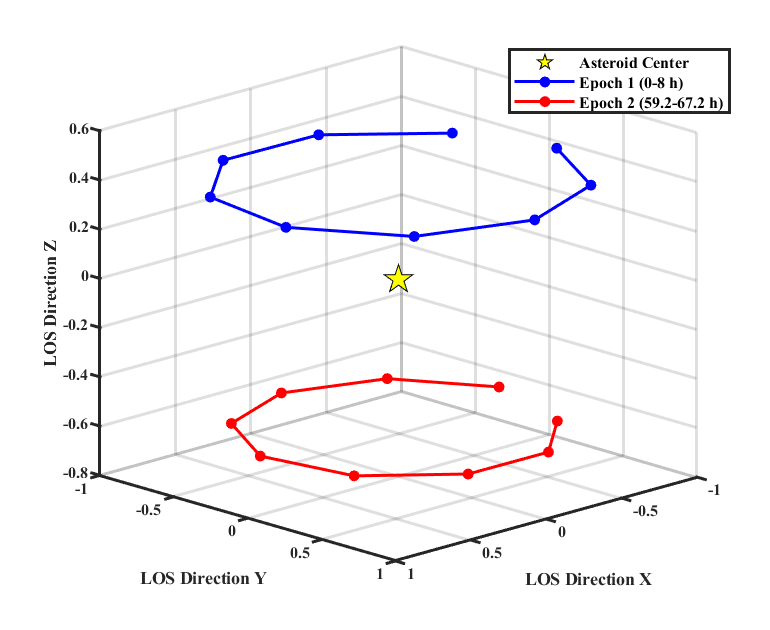
\includegraphics[width=0.6\columnwidth]{fig_radar_los.png}}
	\caption{Radar LOS directions in the asteroid intrinsic coordinate system across two observation epochs.}
	\label{fig_radar_los}
\end{figure}

\begin{table}[htbp]
	\caption{Key Parameters of the ISAR Simulation}
	\label{tab_sim_params}
	\centering
	\renewcommand{\arraystretch}{1.1} % 增加行高，使垂直居中更美观
	\begin{tabular}{|c|l|c|c|}
		\hline
		% 四个表头全部强制居中并加粗
		\multicolumn{1}{|c|}{\textbf{Category}} & 
		\multicolumn{1}{c|}{\textbf{Parameter}} & 
		\multicolumn{1}{c|}{\textbf{Symbol}} & 
		\multicolumn{1}{c|}{\textbf{Value}} \\ \hline
		
		% 使用 multirow{行数}{*}{内容} 实现垂直居中
		\multirow{4}{*}{\shortstack{Target \\ (1999 JV6)}} & Dimensions & ($X, Y, Z$) & 44.39, 21.92, 20.88~m \\ \cline{2-4} 
		& Spin period & $T$ & 9.0~h \\ \cline{2-4} 
		& Rotation axis & ($\lambda, \beta$) & $23.3^{\circ}, 45.0^{\circ}$ \\ \cline{2-4} 
		& Initial phase & $\phi_0$ & $60.0^{\circ}$ \\ \hline
		
		\multirow{4}{*}{\shortstack{Radar \\ System}} & Carrier frequency & $f_c$ & 9.6~GHz \\ \cline{2-4} 
		& Bandwidth & $B$ & 150~MHz \\ \cline{2-4} 
		& Range resolution & $\rho_r$ & 1~m \\ \cline{2-4} 
		& Doppler resolution & $\rho_d$ & 0.01~Hz \\ \hline
		
		\multirow{3}{*}{Observation} & Observation epochs & $N_{ep}$ & 2 \\ \cline{2-4} 
		& Total frames & $N_{fr}$ & 18 \\ \cline{2-4} 
		& SNR & $SNR$ & 16~dB \\ \hline
	\end{tabular}
\end{table}

\subsection{Rotation Parameter Estimation Results}



\subsection{Shape Parameter Inversion Results}

\section{Conclusion}


\section*{Acknowledgment}

The authors would like to acknowledge the JPL for providing the asteroid ephemeris data used in this study. Furthermore, we extend our gratitude to the 3D Asteroid Catalogue for providing the 3D asteroid shape models, which were instrumental in the ISAR imaging simulation and 3D reconstruction experiments.


\bibliographystyle{IEEEtran}
\bibliography{CIE}
\end{document}
